\documentclass[12pt,a4paper]{article}

\usepackage[T1]{fontenc}
\usepackage[utf8]{inputenc} % Use UTF-8 encoding for input
\usepackage[french]{babel}

\usepackage{lmodern}	
\usepackage{amsmath}
\usepackage{amsfonts}
\usepackage{amssymb}
\usepackage{graphicx}
\usepackage{xcolor}
\usepackage{mathtools}
\usepackage{fancyhdr}
\usepackage{enumitem}
\usepackage{tcolorbox}
\usepackage{colortbl}
\usepackage{multirow}
\usepackage{stmaryrd}
\usepackage{dsfont}
\usepackage{tikz}
\usepackage{hyperref}
\usepackage[upgreek]{txgreeks}
\usepackage{algpseudocode}
\usepackage{algorithm}
\usepackage[text={15cm,24.5cm},centering]{geometry}


% Définir le texte affiché en fin de page
\pagestyle{fancy}
\fancyhf{}  % Clear the default headers and footers
\rfoot{\hrule
    \vspace{0.3cm}
    \noindent\textsf{Résolution de systèmes linéaires issus d'EDP}
    \hfill \thepage
}
\renewcommand{\headrulewidth}{0pt}

\title{\vspace{4cm}
        Rapport \\
        \vspace{1cm} \textbf{TP2 : Algèbre Linéaire Creuse} \\ 
        \vspace{4cm} 
}

\author{\textit{Réalisé par} \vspace{0.5cm}\\
         \textbf{Mathilde Ferreira} \\
        \textbf{Félix Foucher de Brandois}
}
        
\date{\vfill
        \textit{ENSEEIHT} - 
        \textit{Formation ModIA, 5$^{e}$ année}
        \hfill
        \textit{2024-2025} \\
        \vspace{1cm}
}


\begin{document}

\begin{figure}[t]
    \centering
    
\includegraphics[width=7cm]{src/inp_n7.png}
    \hfill
    
\includegraphics[width=5.5cm]{src/insa_toulouse.png}
\end{figure}


\maketitle
\thispagestyle{empty}

\newpage


\section{Introduction}

\noindent On cherche à résoudre le système linéaire : $Ax = b$ 
avec $A \in \mathbb{R}^{n \times n}$ une matrice creuse, $b \in \mathbb{R}^{n}$ et $x \in \mathbb{R}^{n}$. \\

Pour cela, nous allons étudier les méthodes directes pour la résolution de systèmes linéaires creux.
Ces méthodes reposent sur des décompositions factorielles telles que la factorisation de Cholesky et la décomposition LU. \\

L'objectif est d'analyser l'impact des réordonnancements sur la structure des matrices et d'optimiser le nombre d'opérations nécessaires à la résolution. \\

Pour évaluer la qualité des solutions calculées, nous utiliserons l'erreur inverse <<normwise>> définie par :
$$
\eta_b^N(\tilde{x}) = \frac{\|b - A\tilde{x}\|}{\|b\|}.
$$

\section{Nombre d'opérations de la phase de résolution}

Dans le cas d'une factorisation de Cholesky d'une matrice symétrique définie positive $A = LL^T$, la résolution du système $Ax = b$ se fait par la résolution des deux systèmes linéaires triangulaires $Ly = b$ puis $L^Tx = y$. \\

\noindent\textbf{Résolution de $Ly = b$ :} \\
Pour résoudre le système $Ly = b$, on utilise une substitution avant.
Si $L$ est creuse, le nombre d'opérations est proportionnel au nombre d'éléments non nuls $nnz(L)$ de $L$. \\
Chaque élément non nul de $L$ contribue à une multiplication et une addition (soustraction) dans le processus de substitution.
Ainsi, le nombre total d'opérations pour résoudre le système $Ly = b$ est approximativement : 
$$
\text{Flops pour } L y = b \approx 2 \cdot \text{nnz}(L).
$$

\noindent\textbf{Résolution de $L^Tx = y$ :} \\
Pour résoudre le système $L^Tx = y$, on utilise une substitution arrière.
Le nombre d'opérations est similaire à celui de la substitution avant, soit approximativement :
$$
\text{Flops pour } L^T x = y \approx 2 \cdot \text{nnz}(L).
$$

Finalement, le nombre total d'opérations pour résoudre le système $Ax = b$ est approximativement :
$$
\text{Flops pour } Ax = b \approx 4 \cdot \text{nnz}(L).
$$

\noindent Le critère pour choisir une permutation est donc de minimiser le nombre de non-zéros de $L$, $nnz(L)$, afin de réduire le coût de la résolution.


\section{Résolution du système linéaire symétrique avec une factorisation
de Cholesky}

On cherche à résoudre le système linéaire : $Ax = b$ où $A$ est une matrice symétrique et $b = (1, 2, \ldots, n)^T$. \\
Nous avons à notre disposition les $4$ matrices \texttt{mat0}, \ldots, \texttt{mat3} qui sont les matrices provenant d’un problème de la chaleur avec différents maillage, ainsi que de la matrice \texttt{BCSSTK27}. \\

Après avoir préalablement vérifié que les matrices étaient symétriques définies positives, nous avons résolu les systèmes avec et sans réordonnancement.

\subsection{Matrice \texttt{mat0}}

\begin{table}[H]
    \centering
    \begin{tabular}{|l|c|c|c|c|c|}
    \hline
    \rowcolor{gray!20} \textbf{Permutation} & \textbf{Normwise Error} & \textbf{Error} & \textbf{FLOPS} & \textbf{Nb Non Zero} & \textbf{Time (s)} \\
    \hline
    \textbf{\textsf{sans permutation}} & $1.2258 \times 10^{-12}$ & $1.0764 \times 10^{-13}$ & 15864 & 7777 & 0.001313 \\
    \hline
    \textbf{\textsf{amd}} & $1.5298 \times 10^{-12}$ & $2.0553 \times 10^{-16}$ & 4720 & 2205 & 0.001393 \\
    \hline
    \textbf{\textsf{colamd}} & $1.717 \times 10^{-12}$ & $1.5064 \times 10^{-14}$ & 5468 & 2579 & 0.006841 \\
    \hline
    \textbf{\textsf{symamd}} & $1.2042 \times 10^{-12}$ & $1.182 \times 10^{-13}$ & 4744 & 2217 & 0.000851 \\
    \hline
    \textbf{\textsf{symrcm}} & $1.4392 \times 10^{-12}$ & $9.5756 \times 10^{-14}$ & 6248 & 2969 & 0.002007 \\
    \hline
    \textbf{\textsf{colperm}} & $9.3378 \times 10^{-13}$ & $1.6504 \times 10^{-13}$ & 12812 & 6251 & 0.003066 \\
    \hline
    \end{tabular}
    \caption{Tableau des résultats pour la matrice \texttt{mat0}}
\end{table}

La permutation \textsf{symamd} est celle qui minimise le nombre de non-zéros de $L$ et le nombre d'opérations nécessaires à la résolution du système.
Elle permet d'obtenir une erreur inverse $\eta_b^N(\tilde{x}) = 1.2042 \times 10^{-12}$ : la solution est donc très proche de la solution exacte. \\

La figure \ref{fig:mat0} montre la structure de la matrice $A$ obtenue après la factorisation de Cholesky avec la permutation \textsf{symamd}.

\begin{figure}[H]
    \centering
    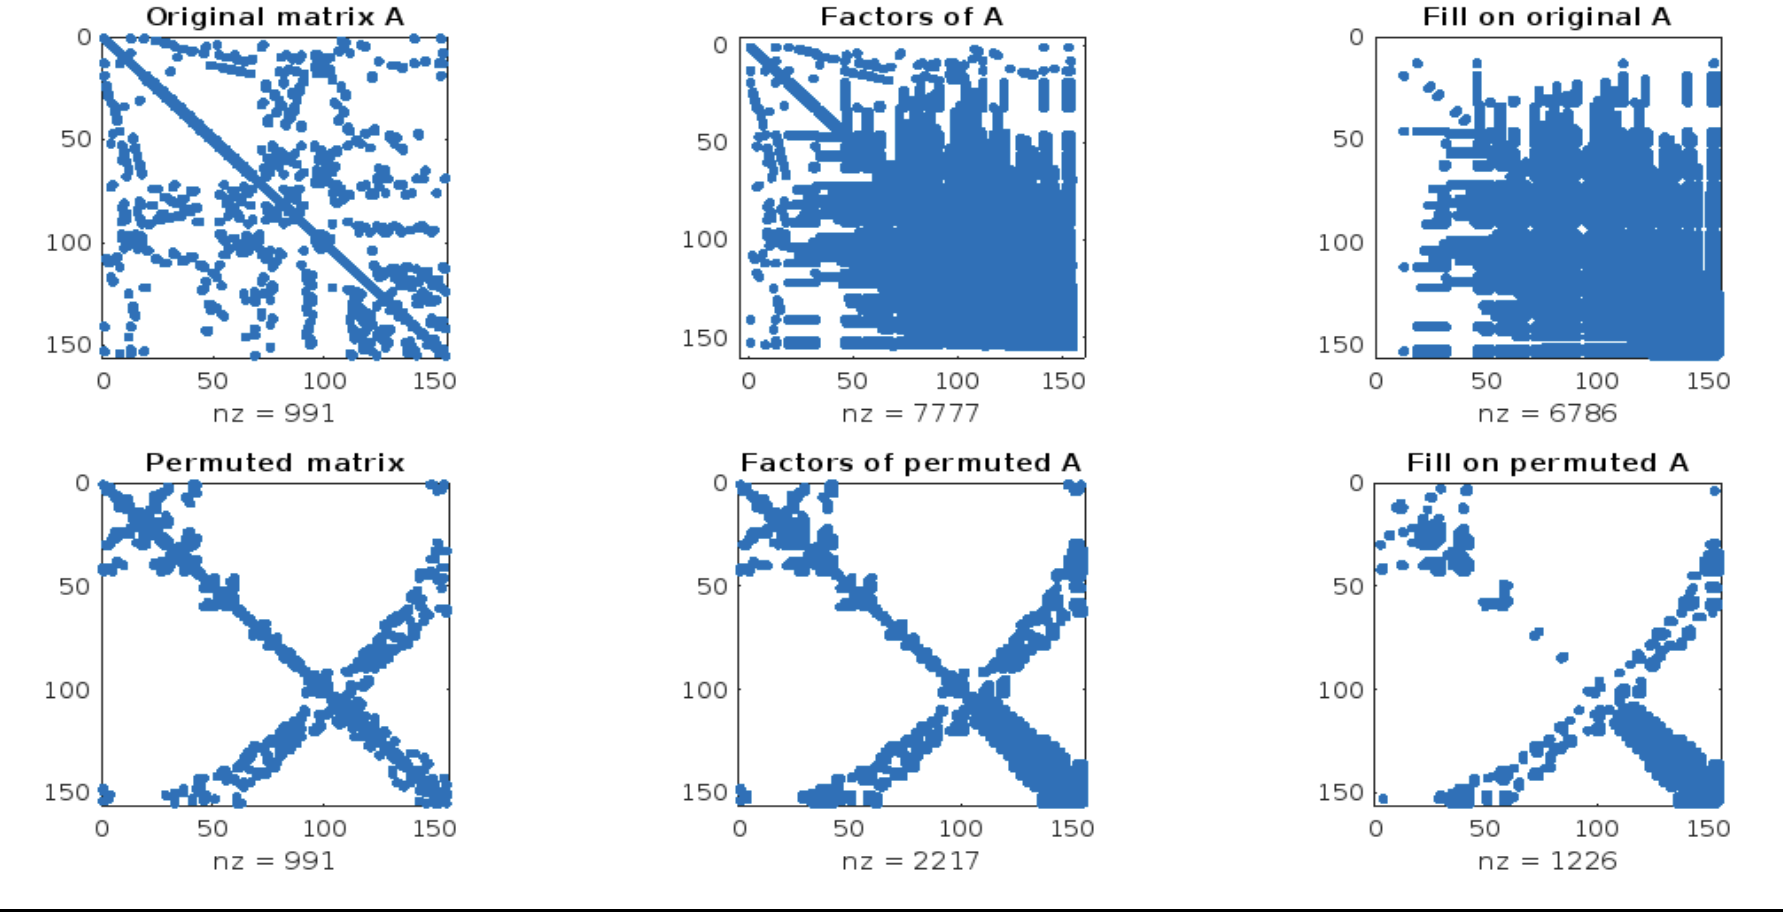
\includegraphics[width=0.6\textwidth]{src/mat0_symamd.png}
    \caption{Structure de la matrice $A$ pour la matrice \texttt{mat0} avec la permutation \textsf{symamd}}
    \label{fig:mat0}
\end{figure}

\subsection{Matrice \texttt{mat1}}

\begin{table}[H]
    \centering
    \begin{tabular}{|l|c|c|c|c|c|}
    \hline
    \rowcolor{gray!20} \textbf{Permutation} & \textbf{Normwise Error} & \textbf{Error} & \textbf{FLOPS} & \textbf{Nb Non Zero} & \textbf{Time (s)} \\
    \hline
    \textbf{\textsf{sans permutation}} & $7.5124 \times 10^{-12}$ & $4.495 \times 10^{-13}$ & $1.4233 \times 10^{5}$ & 70591 & 0.001822 \\
    \hline
    \textbf{\textsf{amd}} & $5.5497 \times 10^{-12}$ & $7.4669 \times 10^{-16}$ & 28104 & 13479 & 0.00147 \\
    \hline
    \textbf{\textsf{colamd}} & $8.0905 \times 10^{-12}$ & $1.5368 \times 10^{-13}$ & 35144 & 16999 & 0.004453 \\
    \hline
    \textbf{\textsf{symamd}} & $7.7481 \times 10^{-12}$ & $1.2991 \times 10^{-13}$ & 28192 & 13523 & 0.001385 \\
    \hline
    \textbf{\textsf{symrcm}} & $8.7598 \times 10^{-12}$ & $2.7061 \times 10^{-13}$ & 42224 & 20539 & 0.001671 \\
    \hline
    \textbf{\textsf{colperm}} & $6.989 \times 10^{-12}$ & $8.7731 \times 10^{-14}$ & $1.45 \times 10^{5}$ & 71927 & 0.003352 \\
    \hline
    \end{tabular}
    \caption{Tableau des résultats pour la matrice \texttt{mat1}}
\end{table}

La permutation \textsf{amd} est celle qui minimise le nombre de non-zéros de $L$ et le nombre d'opérations nécessaires à la résolution du système.
Elle permet d'obtenir une erreur inverse $\eta_b^N(\tilde{x}) = 5.5497 \times 10^{-12}$. \\

La figure \ref{fig:mat1} montre la structure de la matrice $A$ obtenue après la factorisation de Cholesky avec la permutation \textsf{amd}.
\begin{figure}[H]
    \centering
    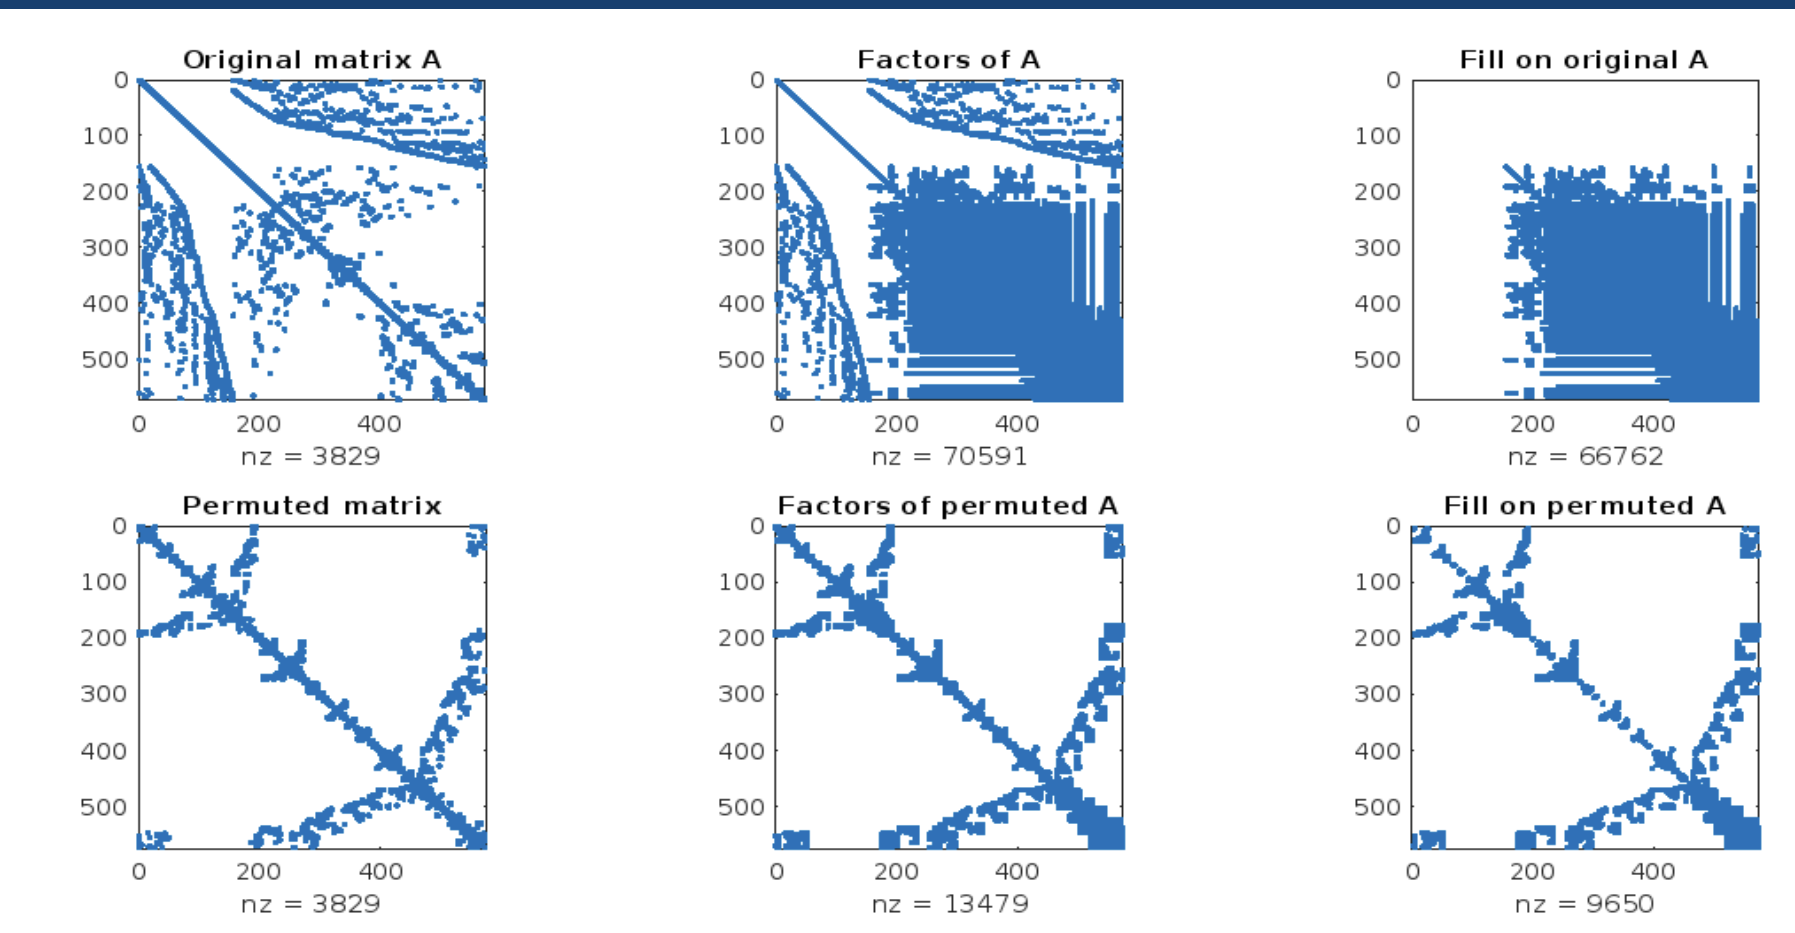
\includegraphics[width=0.6\textwidth]{src/mat1_amd.png}
    \caption{Structure de la matrice $A$ pour la matrice \texttt{mat1} avec la permutation \textsf{amd}}
    \label{fig:mat1}
\end{figure}

\subsection{Matrice \texttt{mat2}}

\begin{table}[H]
    \centering
    \begin{tabular}{|l|c|c|c|c|c|}
    \hline
    \rowcolor{gray!20} \textbf{Permutation} & \textbf{Normwise Error} & \textbf{Error} & \textbf{FLOPS} & \textbf{Nb Non Zero} & \textbf{Time (s)} \\
    \hline
    \textbf{\textsf{sans permutation}} & $3.0112 \times 10^{-11}$ & $5.8446 \times 10^{-13}$ & $1.3116 \times 10^{6}$ & $6.5358 \times 10^{5}$ & 0.010638 \\
    \hline
    \textbf{\textsf{amd}} & $2.7188 \times 10^{-11}$ & $6.4422 \times 10^{-14}$ & $1.7513 \times 10^{5}$ & 85363 & 0.004498 \\
    \hline
    \textbf{\textsf{colamd}} & $3.0935 \times 10^{-11}$ & $1.0542 \times 10^{-12}$ & $2.0152 \times 10^{5}$ & 98557 & 0.00864 \\
    \hline
    \textbf{\textsf{symamd}} & $3.099 \times 10^{-11}$ & $7.6133 \times 10^{-13}$ & $1.661 \times 10^{5}$ & 80851 & 0.003753 \\
    \hline
    \textbf{\textsf{symrcm}} & $4.2393 \times 10^{-11}$ & $1.1391 \times 10^{-12}$ & $3.076 \times 10^{5}$ & $1.516 \times 10^{5}$ & 0.004124 \\
    \hline
    \textbf{\textsf{colperm}} & $2.9388 \times 10^{-11}$ & $1.0891 \times 10^{-12}$ & $1.277 \times 10^{6}$ & $6.363 \times 10^{5}$ & 0.013823 \\
    \hline
    \end{tabular}
    \caption{Tableau des résultats pour la matrice \texttt{mat2}}
\end{table}

La permutation \textsf{symamd} est celle qui minimise le nombre de non-zéros de $L$ et le nombre d'opérations nécessaires à la résolution du système.
Elle permet d'obtenir une erreur inverse $\eta_b^N(\tilde{x}) = 3.099 \times 10^{-11}$. \\

La figure \ref{fig:mat2} montre la structure de la matrice $A$ obtenue après la factorisation de Cholesky avec la permutation \textsf{symamd}.
\begin{figure}[H]
    \centering
    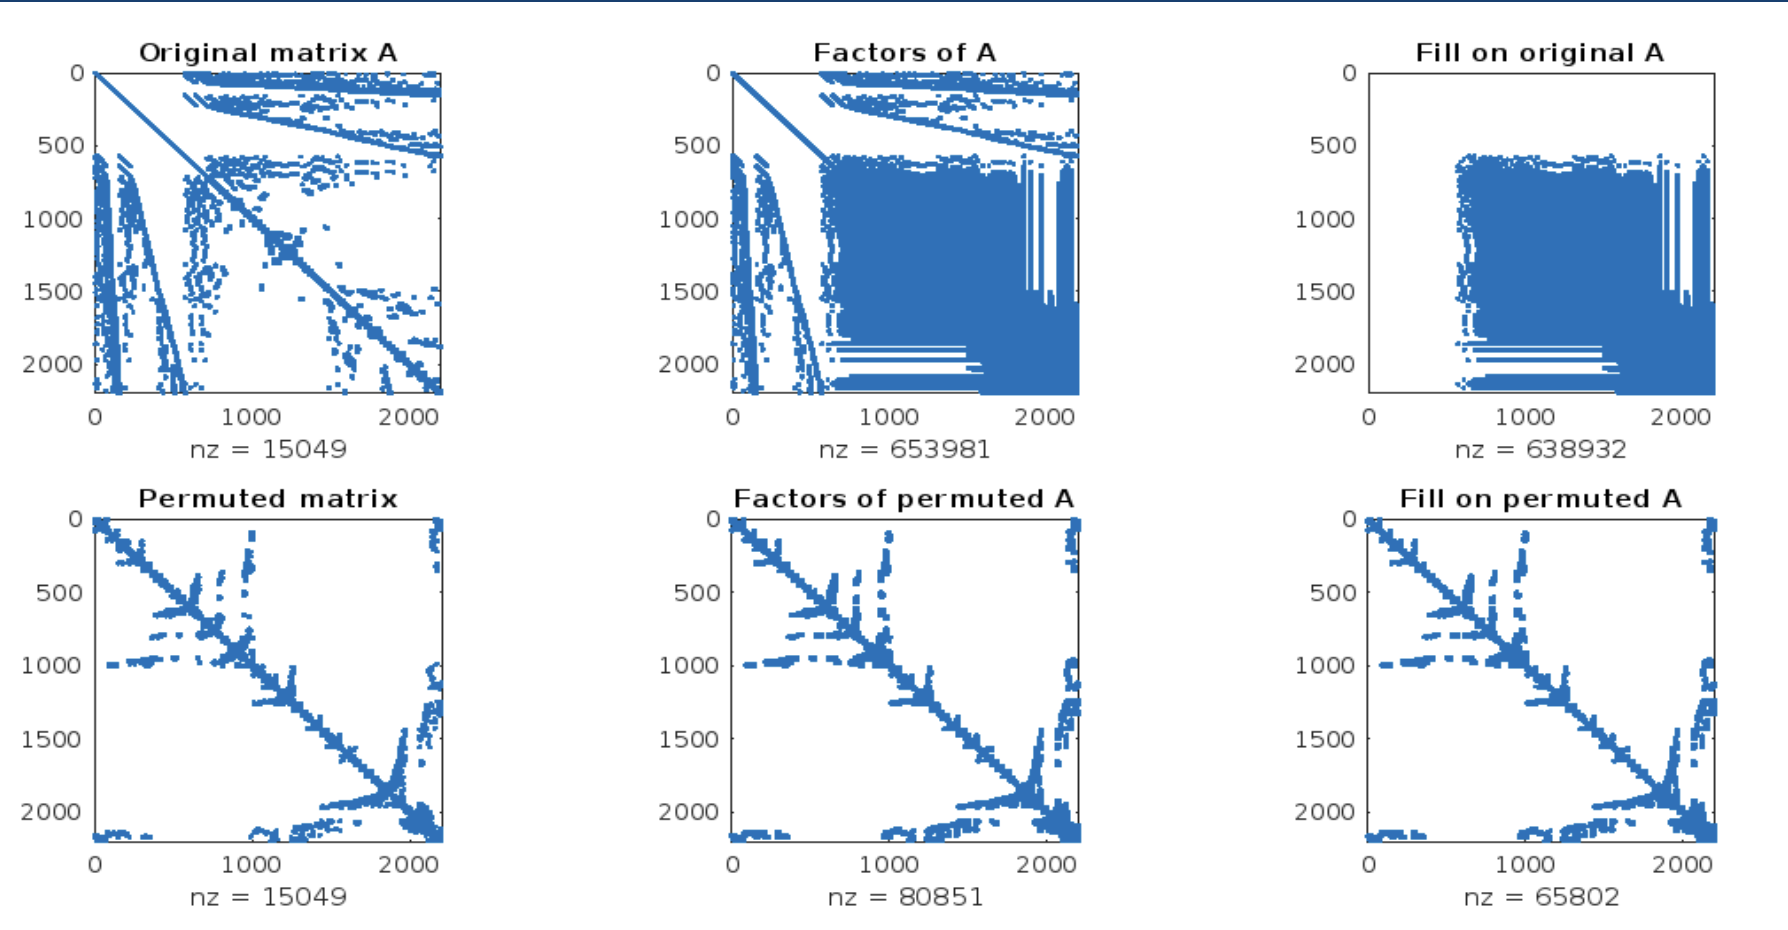
\includegraphics[width=0.6\textwidth]{src/mat2_symamd.png}
    \caption{Structure de la matrice $A$ pour la matrice \texttt{mat2} avec la permutation \textsf{symamd}}
    \label{fig:mat2}
\end{figure}

\subsection{Matrice \texttt{mat3}}

\begin{table}[H]
    \centering
    \begin{tabular}{|l|c|c|c|c|c|}
    \hline
    \rowcolor{gray!20} \textbf{Permutation} & \textbf{Normwise Error} & \textbf{Error} & \textbf{FLOPS} & \textbf{Nb Non Zero} & \textbf{Time (s)} \\
    \hline
    \textbf{\textsf{sans permutation}} & $1.2946 \times 10^{-10}$ & $1.5834 \times 10^{-12}$ & $1.1257 \times 10^{7}$ & $5.6199 \times 10^{6}$ & 0.11676 \\
    \hline
    \textbf{\textsf{amd}} & $1.169 \times 10^{-10}$ & $1.4303 \times 10^{-13}$ & $1.0218 \times 10^{6}$ & $5.0227 \times 10^{5}$ & 0.015098 \\
    \hline
    \textbf{\textsf{colamd}} & $1.2809 \times 10^{-10}$ & $2.444 \times 10^{-12}$ & $1.2247 \times 10^{6}$ & $6.0372 \times 10^{5}$ & 0.026894 \\
    \hline
    \textbf{\textsf{symamd}} & $1.0873 \times 10^{-10}$ & $1.5197 \times 10^{-12}$ & $9.249 \times 10^{5}$ & $4.5382 \times 10^{5}$ & 0.014656 \\
    \hline
    \textbf{\textsf{symrcm}} & $1.7213 \times 10^{-10}$ & $3.3079 \times 10^{-12}$ & $2.3614 \times 10^{6}$ & $1.1721 \times 10^{6}$ & 0.015146 \\
    \hline
    \textbf{\textsf{colperm}} & $1.2655 \times 10^{-10}$ & $3.7064 \times 10^{-13}$ & $1.0509 \times 10^{7}$ & $5.246 \times 10^{6}$ & 0.11473 \\
    \hline
    \end{tabular}
    \caption{Tableau des résultats pour la matrice \texttt{mat3}}
\end{table}

La permutation \textsf{symamd} est celle qui minimise le nombre de non-zéros de $L$ et le nombre d'opérations nécessaires à la résolution du système.
Elle permet d'obtenir une erreur inverse $\eta_b^N(\tilde{x}) = 1.0873 \times 10^{-10}$. \\

La figure \ref{fig:mat3} montre la structure de la matrice $A$ obtenue après la factorisation de Cholesky avec la permutation \textsf{symamd}.
\begin{figure}[H]
    \centering
    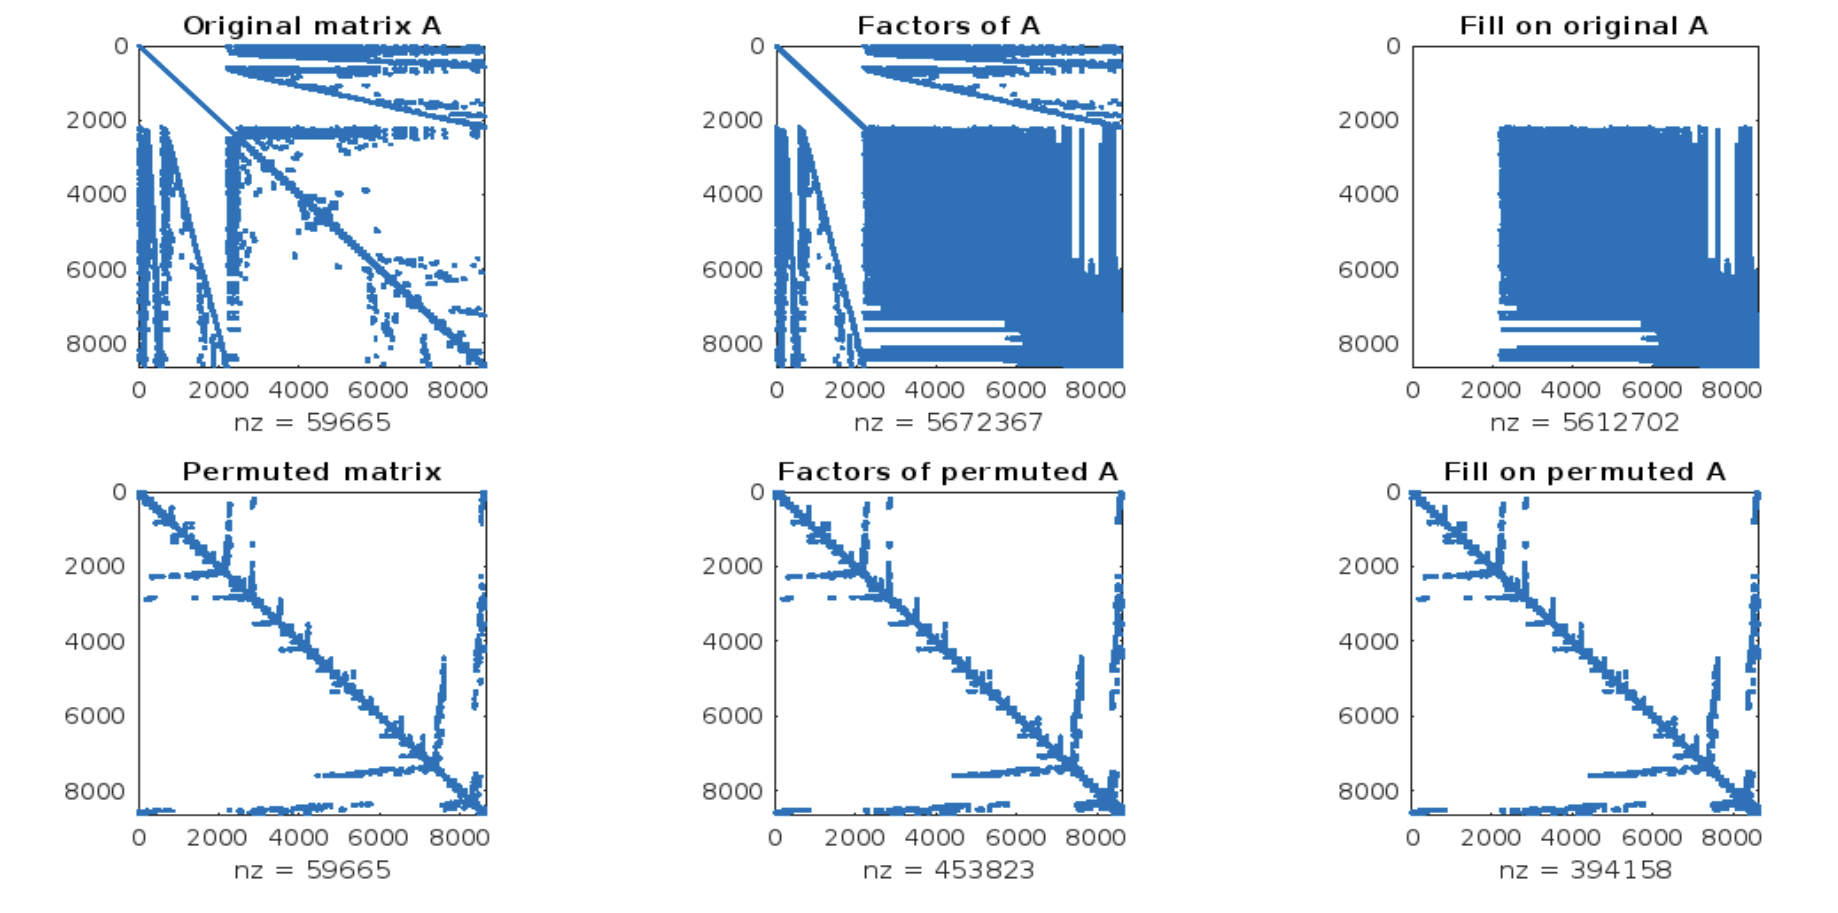
\includegraphics[width=0.6\textwidth]{src/mat3_symamd.png}
    \caption{Structure de la matrice $A$ pour la matrice \texttt{mat3} avec la permutation \textsf{symamd}}
    \label{fig:mat3}
\end{figure}

\subsection{Matrice \texttt{BCSSTK27}}

\begin{table}[H]
    \centering
    \begin{tabular}{|l|c|c|c|c|c|}
    \hline
    \rowcolor{gray!20} \textbf{Permutation} & \textbf{Normwise Error} & \textbf{Error} & \textbf{FLOPS} & \textbf{Nb Non Zero} & \textbf{Time (s)} \\
    \hline
    \textbf{\textsf{sans permutation}} & $3.6069 \times 10^{-14}$ & $7.3934 \times 10^{-15}$ & $2.0206 \times 10^{5}$ & $9.9806 \times 10^{4}$ & 0.002375 \\
    \hline
    \textbf{\textsf{amd}} & $3.6027 \times 10^{-14}$ & $2.4155 \times 10^{-15}$ & $2.23 \times 10^{5}$ & $1.1027 \times 10^{5}$ & 0.004195 \\
    \hline
    \textbf{\textsf{colamd}} & $3.8606 \times 10^{-14}$ & $8.2324 \times 10^{-15}$ & $2.0566 \times 10^{5}$ & $1.016 \times 10^{5}$ & 0.006406 \\
    \hline
    \textbf{\textsf{symamd}} & $4.494 \times 10^{-14}$ & $6.9124 \times 10^{-15}$ & $2.3542 \times 10^{5}$ & $1.1649 \times 10^{5}$ & 0.004641 \\
    \hline
    \textbf{\textsf{symrcm}} & $3.5509 \times 10^{-14}$ & $4.8157 \times 10^{-15}$ & $2.035 \times 10^{5}$ & $1.0053 \times 10^{5}$ & 0.003569 \\
    \hline
    \textbf{\textsf{colperm}} & $4.0717 \times 10^{-14}$ & $9.7507 \times 10^{-15}$ & $1.314 \times 10^{6}$ & $6.5577 \times 10^{5}$ & 0.010103 \\
    \hline
    \end{tabular}
    \caption{Tableau des résultats pour la matrice \texttt{BCSSTK27}}
\end{table}

L'absence de permutation minimise le nombre de non-zéros de $L$ et le nombre d'opérations nécessaires à la résolution du système.
Elle permet d'obtenir une erreur inverse $\eta_b^N(\tilde{x}) = 3.6069 \times 10^{-14}$. \\

La figure \ref{fig:bcsstk27} montre la structure de la matrice $A$ obtenue après la factorisation de Cholesky sans permutation, ainsi qu'avec la permutation \textsf{symrcm} (qui donne des résultats similaires).
\begin{figure}[H]
    \centering
    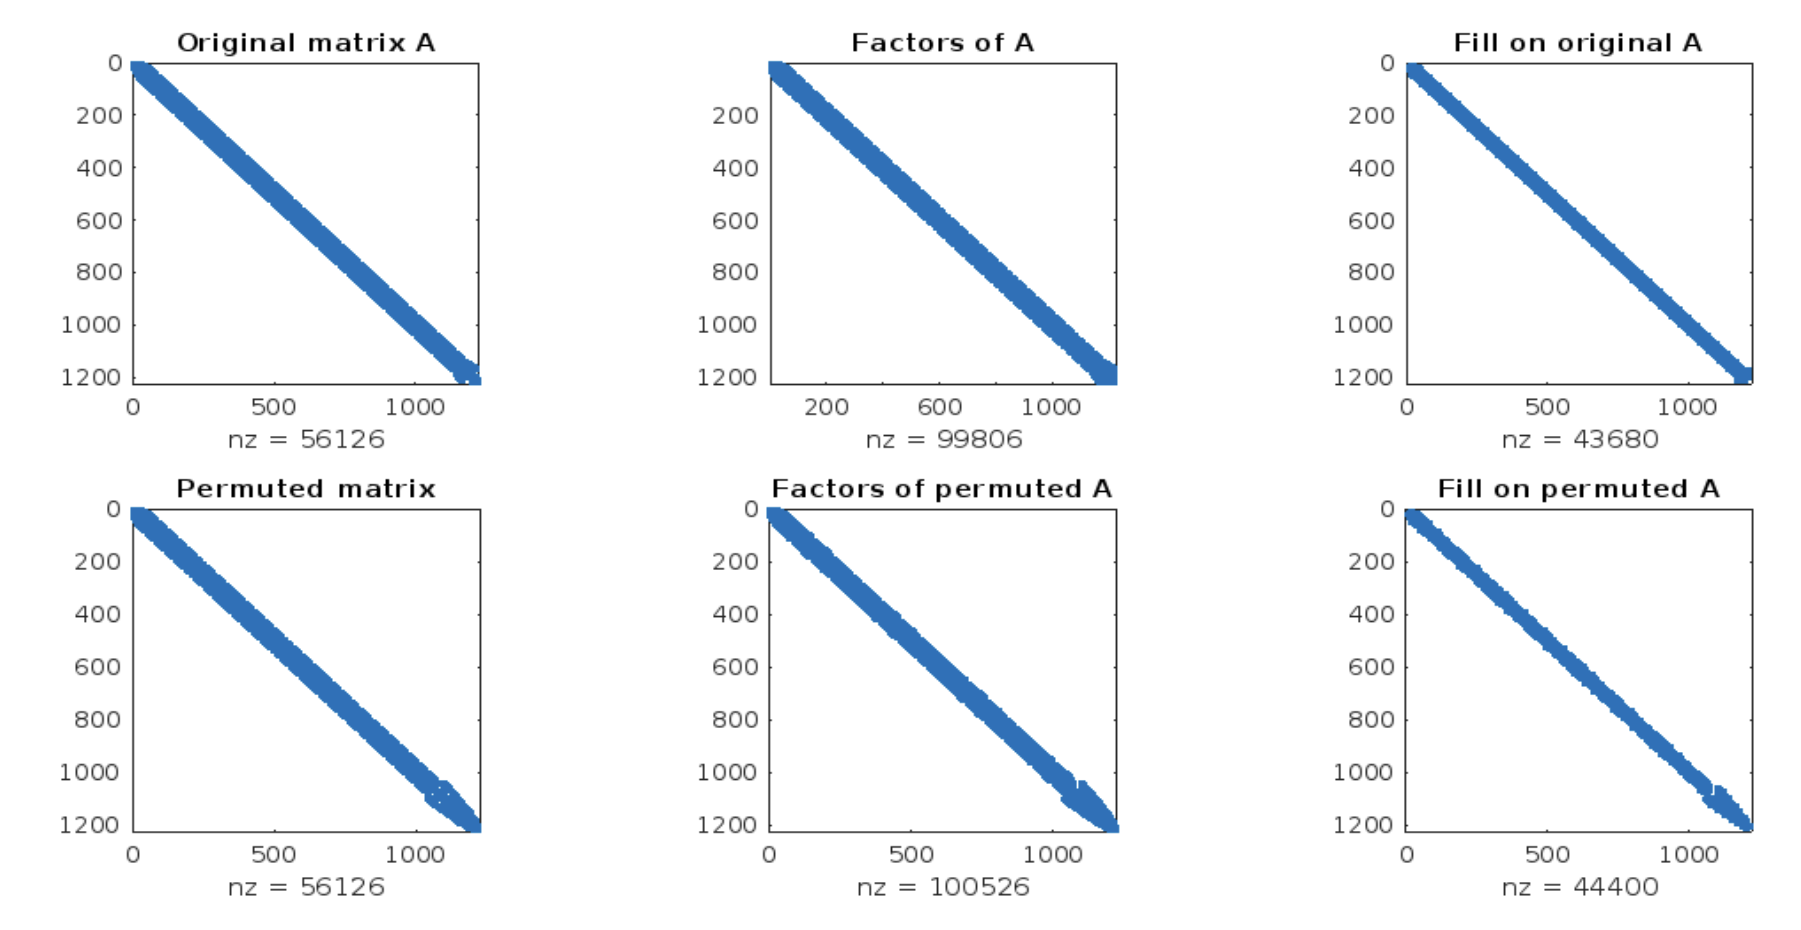
\includegraphics[width=0.6\textwidth]{src/bcsstk27_symrcm.png}
    \caption{Structure de la matrice $A$ pour la matrice \texttt{BCSSTK27} sans permutation}
    \label{fig:bcsstk27}
\end{figure}


\end{document}